% !TEX encoding = UTF-8
% !TEX program = pdflatex
% !TeX spellcheck = en_GB
% !BIB = biber

\documentclass[english]{article}
\usepackage{amsmath}
\usepackage{wasysym}
\usepackage{amssymb}
\usepackage{subcaption}
\usepackage{babel}
\usepackage[utf8]{inputenc}
\usepackage{graphicx}
\usepackage[obeyspaces]{url}

\usepackage{titlesec}

\setcounter{secnumdepth}{4}

\titleformat{\paragraph}
{\normalfont\normalsize\bfseries}{\theparagraph}{1em}{}
\titlespacing*{\paragraph}
{0pt}{3.25ex plus 1ex minus .2ex}{1.5ex plus .2ex}

\graphicspath{{./images/}}
\usepackage{hyperref}
\hypersetup{
    colorlinks=true, 
	linkcolor=blue, 
	filecolor=blue, 
	citecolor = black,       
	urlcolor=blue, 
}
\usepackage{listings}
\lstset{
  xleftmargin=15pt,
  xrightmargin=0pt,
  framexleftmargin=0pt,
  framexrightmargin=0pt,
  basicstyle={\fontsize{9pt}{10pt}\ttfamily},
  columns=flexible,
  numbers=left,
  numbersep=10pt,
  numberstyle={\fontsize{9pt}{11pt}\selectfont\color[rgb]{0.4,0.4,0.1}},
  keepspaces=true,
  showstringspaces=false,
  identifierstyle=\color[rgb]{0.1,0.1,0.1},
  keywordstyle=\color{blue},
  commentstyle=\color[rgb]{0,0.3,0},
  morekeywords={rule, lemma},
  morekeywords=[2]{let, in},
  morekeywords=[3]{Fr, pk},
  morekeywords=[4]{In, Out},
  morekeywords=[5]{senc, aenc, h}
  morecomment=[s][keywordstyle3]{/*}{/},
  keywordstyle=\color[rgb]{0.44,0.57,0.65},
  stringstyle=\color{green},
  keywordstyle=[2]{\color[rgb]{0.86,0.57,0.18}},
  keywordstyle=[3]{\bfseries\color[rgb]{0,0.3,0.2}}
  }
\usepackage{biblatex}
\addbibresource{thud.bib}

\title{An overview and analysis of Apple’s AirTag technology and FindMy service}
\author{Zanolin Lorenzo}
\date{February, 2024}
\begin{document}

\maketitle

\tableofcontents
\newpage

% scaletta:
% UWB, spiegazione generica di come funziona
% UWB analisi sulla sicurezza implementata da Apple
% FindMy spiegazione dell'architettura
% FindMy spiego ogni singola funzionalità
% FindMy esempio di come viene localizzato un oggetto (U1-uwb and BLE)
% AirTag analisi della sicurezza
% AirTag analisi caso stalking e come ovviare il problema
% AirTag esempio di funzionamento
% AirTag possibili utilizzi futuri

\begin{abstract}
  The main goal of this project is to dig into how Apple AirTags work, including their setup, security measures, and uses; since everything is tied to the FindMy network and the UWB technology, we will also look into the security methods used in this network and the basic principle of the Ultra-Wideband (UWB). The idea is to get a clear picture of how Apple AirTags are put together, how secure they are, and the different ways they're used in the FindMy network.
\end{abstract}

\section{Introduction}\label{sec:intro}
In the rapidly evolving landscape of technological advancements, Apple's AirTags have emerged as an innovation, offering a solution to tracking and locating personal belongings. This paper delves into the architecture and security of AirTags, with a particular emphasis on the UWB technology that underlies their functionality. Moreover, as AirTags operate within the framework of the FindMy network, this exploration extends to an overview of the security measures embedded in both the device and the overarching network; through the examination of the relationship between AirTags, UWB, and FindMy security, this paper seeks to provide insights of the working principles of the ecosystem which enables accurate location tracking, while also addressing concerns related to privacy and data security.

We will go over the fundamentals of UWB technology in Section \ref{sec:uwb} and examine its benefits from a security standpoint. In Section \ref{sec:find}, we will delve deeper into the examination of the FindMy network. We will begin with providing a general overview of the architecture, go on to a functioning example and end with a security analysis of the whole thing. Lastly, we will conduct a thorough examination of the AirTag concept in Chapter \ref{sec:at}, concentrating on the architecture (first examining the software component, then the hardware component) and then moving on to the security analysis of this technology.

\section{UWB}\label{sec:uwb}
\subsection{Overview}
Within the domain of wireless communication technologies, UWB operates by employing extremely low-power, short-duration pulses that span a broad spectrum, allowing for high data transfer rates and precise positioning capabilities. Originally conceived for military and radar applications, it has gradually invaded diverse sectors, finding particular prominence in consumer electronics, healthcare, automotive systems, and the Internet of Things (IoT).

The unique feature of UWB is its capacity to send information across a large frequency range, usually several gigahertz; a UWB transmitter sends billions of radio pulses across the wide spectrum frequency and a UWB receiver then translates the pulses into data. The shorter the duration of the impulse, the more precise the distance measurement will be. According to \cite{Coppens2022}, UWB achieves real-time accuracy because the receiver can determine the time of arrival of the signal, allowing centimeter-level accurate ranging using techniques such as Time-of-Flight (ToF), Time Difference of Arrival (TDoA) and Two-Way Ranging (TWR). Combining
this with error correction techniques, the ranging error can
be as low as 58 mm.

Because of its wide spectrum utilization, UWB can coexist peacefully with other wireless technologies and send out massive volumes of data quickly.  Since its ability to transmit info across a wide radio bandwidth, from 500 MHz to several gigahertz, this technology has a short range of operation. According to \cite{di2006uwb}, due to the low energy density and the pseudo-random (PR) characteristics of the transmitted signal, the UWB signal is noise-like which makes unintended detection difficult. To increase UWB’s range and reception reliability, a \textit{MIMO} (multiple-input and multiple-output), distributed antenna system has been added to the standard that enables short-range networks. The antennas can be embedded into a smartphone or other devices such as a wristband or smart key.

According to \cite{aps}, Apple-designed U1 chip uses UWB technology for spatial awareness, allowing iPhone 11, iPhone 11 Pro and iPhone 11 Pro Max or later iPhone models to precisely locate other U1-equipped Apple devices.
When two U1 devices come close to eachother, the two start measuring their exact distance. The ranging is accomplished through Time of Flight (ToF), which is the time it takes for a pulse to get from point A to point B. According to IEEE 802.15.4a \cite{5394030}, UWB can determine the relative position of other devices in the line of sight even up to 200 meters.

A difference w.r.t. Bluetooth Low Energy (BLE) is that with BLE you can’t really measure location or distance. What you can do is to detect if a device like a smartphone is within a range of another device. UWB, in comparison, provides a much higher accuracy (up to a few centimeters). In contrast to BLE, the distance it measures is not based on the signal strength, but the time it takes the signal to travel from point A (smartphone) to point B (UWB tag). Table \ref{tableu} represent the principal differences between the two technologies, data is taken from \cite{encstore}:
\begin{table}[h] 
\caption{BLE-UWB comparison.}
  \centering
  
    \begin{tabular}{l|l|l|}
      \cline{2-3}
      {}                               & {\textbf{UWB}}                & { \textbf{Bluetooth (BLE Beacons)}} \\ \hline
      \multicolumn{1}{|l|}{{  \textbf{Battery}}}  & {  Low consumption}             & {  Low consumption}                  \\ \hline
      \multicolumn{1}{|l|}{{  \textbf{Data Rate}}}  & { 1 Gbps }             & { 2 Mbps }                  \\ \hline
      \multicolumn{1}{|l|}{{  \textbf{Range}}}    & {  up to 200 meters} & {  up to 100 meters}       \\ \hline
      \multicolumn{1}{|l|}{{  \textbf{Accuracy}}} & {  10 centimeters} & {  up to a meter}                    \\ \hline
      \multicolumn{1}{|l|}{{  \textbf{Cost}}}     & {  Low}                         & {Depend on the context }                              \\ \hline
    \end{tabular}
    \label{tableu}
  \end{table}

\subsection{Security analysis}
The fact that UWB pulses are resistant to the multipath effect\footnote{Multipath interference occurs when a signal from a transmitter arrives at a receiver via two or more routes; typically there is a direct path plus a number of indirect paths caused by reflections} is one of its key characteristics. This occurs when radio waves are reflected or refracted by artificial or natural objects near to the primary signal channel, causing the signal to reach the receiver via many paths. Positioning accuracy is improved by immunity to the multipath effect, particularly when compared to other technologies that are more vulnerable. Moreover, UWB's resilience to jamming and narrowband fading makes it a particularly reliable technology choice, even when several UWB systems are being used at once.

Another important aspect to consider is the resistance from Relay Attacks, which is a vulnerability of the majority of signals-based architectures. Within these attacks, the goal is to trick a car into thinking the key and owner are close by using two people with hacking devices \cite{renesas}. The first relays signals from the car to the second thief, who transmits the signal to the house. The key responds, allowing entry into the car. The relay attack intercepts and amplifies wireless signals used to unlock the door and start the car, despite the key's distance. With UWB that would not be possible due to its working scheme: to ensure the car doesn't have to make assumptions, rapid measurements are utilized to establish distance very precisely. Any attempt to relay attack or intercept the UWB signal will merely cause the answering device's acknowledgement signals to arrive later, indicating to the UWB-based lock and ignition that the responding device is actually farther away rather than closer. The car's presumption is replaced with assurance when using UWB, which greatly increases the security of the passive keyless entry system.

The implemented security measures, taken by Apple, are the following: MAC address randomization and frame sequence number randomization \cite{aps}.

\subsubsection{MAC address randomization}
Apple platforms use a randomized media access control address (MAC address) when performing scans when not associated with another device. Because a device’s MAC address changes when disconnected from another device, it can’t be used to persistently track a device by passive observers of traffic.

\subsubsection{Frame sequence number randomization}
Apple devices randomize the sequence numbers whenever a MAC address is changed to a new randomized address.

\section{FindMy network}\label{sec:find}
\subsection{Overview}
Apple created the technology, known as the FindMy network, which is intended to assist consumers in finding their compatible third-party accessories, such as Apple AirTags, as well as their Apple devices, including iPhones, iPads, Macs, and AirPods. By utilizing UWB and BLE technologies, the FindMy network facilitates accurate and instantaneous location tracking.

Because it may be used to find everything you need to, Apple combined the Find My Friends and Find My iPhone apps into a single one that is simply called \textit{Find My}. Subsequently, Apple has consistently enhanced the Find My app, incorporating functionalities such as monitoring when a iPhone is disconnected, when it is turned off and when it has been wiped.

The app is organized into several sections, accessible by tapping the tabs at the bottom. On the left, you can find people, in the middle, you can find your own devices and items, such as AirTags and Find My-enabled Bluetooth items; finally on the right there's a \textit{Me} tab with all of your settings and info, as we can see in Figure \ref{findmy2}.

There are several useful features within this app, as example:
\begin{itemize}
  \item \textit{Separation alerts}: Designed to let you know if you leave an Apple device, a device attached to an AirTag, or a Find My-enabled third-party device behind.
  \item \textit{Locating friends and sharing location}: Implemented to locate friends and family members that have shared their location with you. You can view their location using the \textit{People} tab within the Find My app.
  \item \textit{Locating devices without connection}: Lets your lost devices be located even when not connected to WiFi or LTE by leveraging BLE and proximity to other nearby Apple devices. When your lost device is offline but close to another one, it's able to connect to that other device over Bluetooth and relay its location. We will come back on this\ldots
  % ovviamente se il bluetooth è off allora non è rilevabile, non basta avere il chip U1 alimentato
  \item \textit{Anti-stalking measures}: Designed to let you know if there's a Bluetooth item near you. You will receive a notification when an unknown item is found and moving with you, so you can make sure no one slips an AirTag or other Find My Bluetooth devices into your things to track you. We will also come back on this following the studies done in \cite{airguard}.
  \item \textit{Precision finding}: Takes advantage of the U1 chip within AirTags and the iPhone 13, iPhone 12 and iPhone 11 models. Apple's U1 chip uses UWB to precisely locate and communicate with other U1-equipped devices, enabling AirTags and iPhones to work together.
\end{itemize}

\begin{figure}[t]
	\centering
	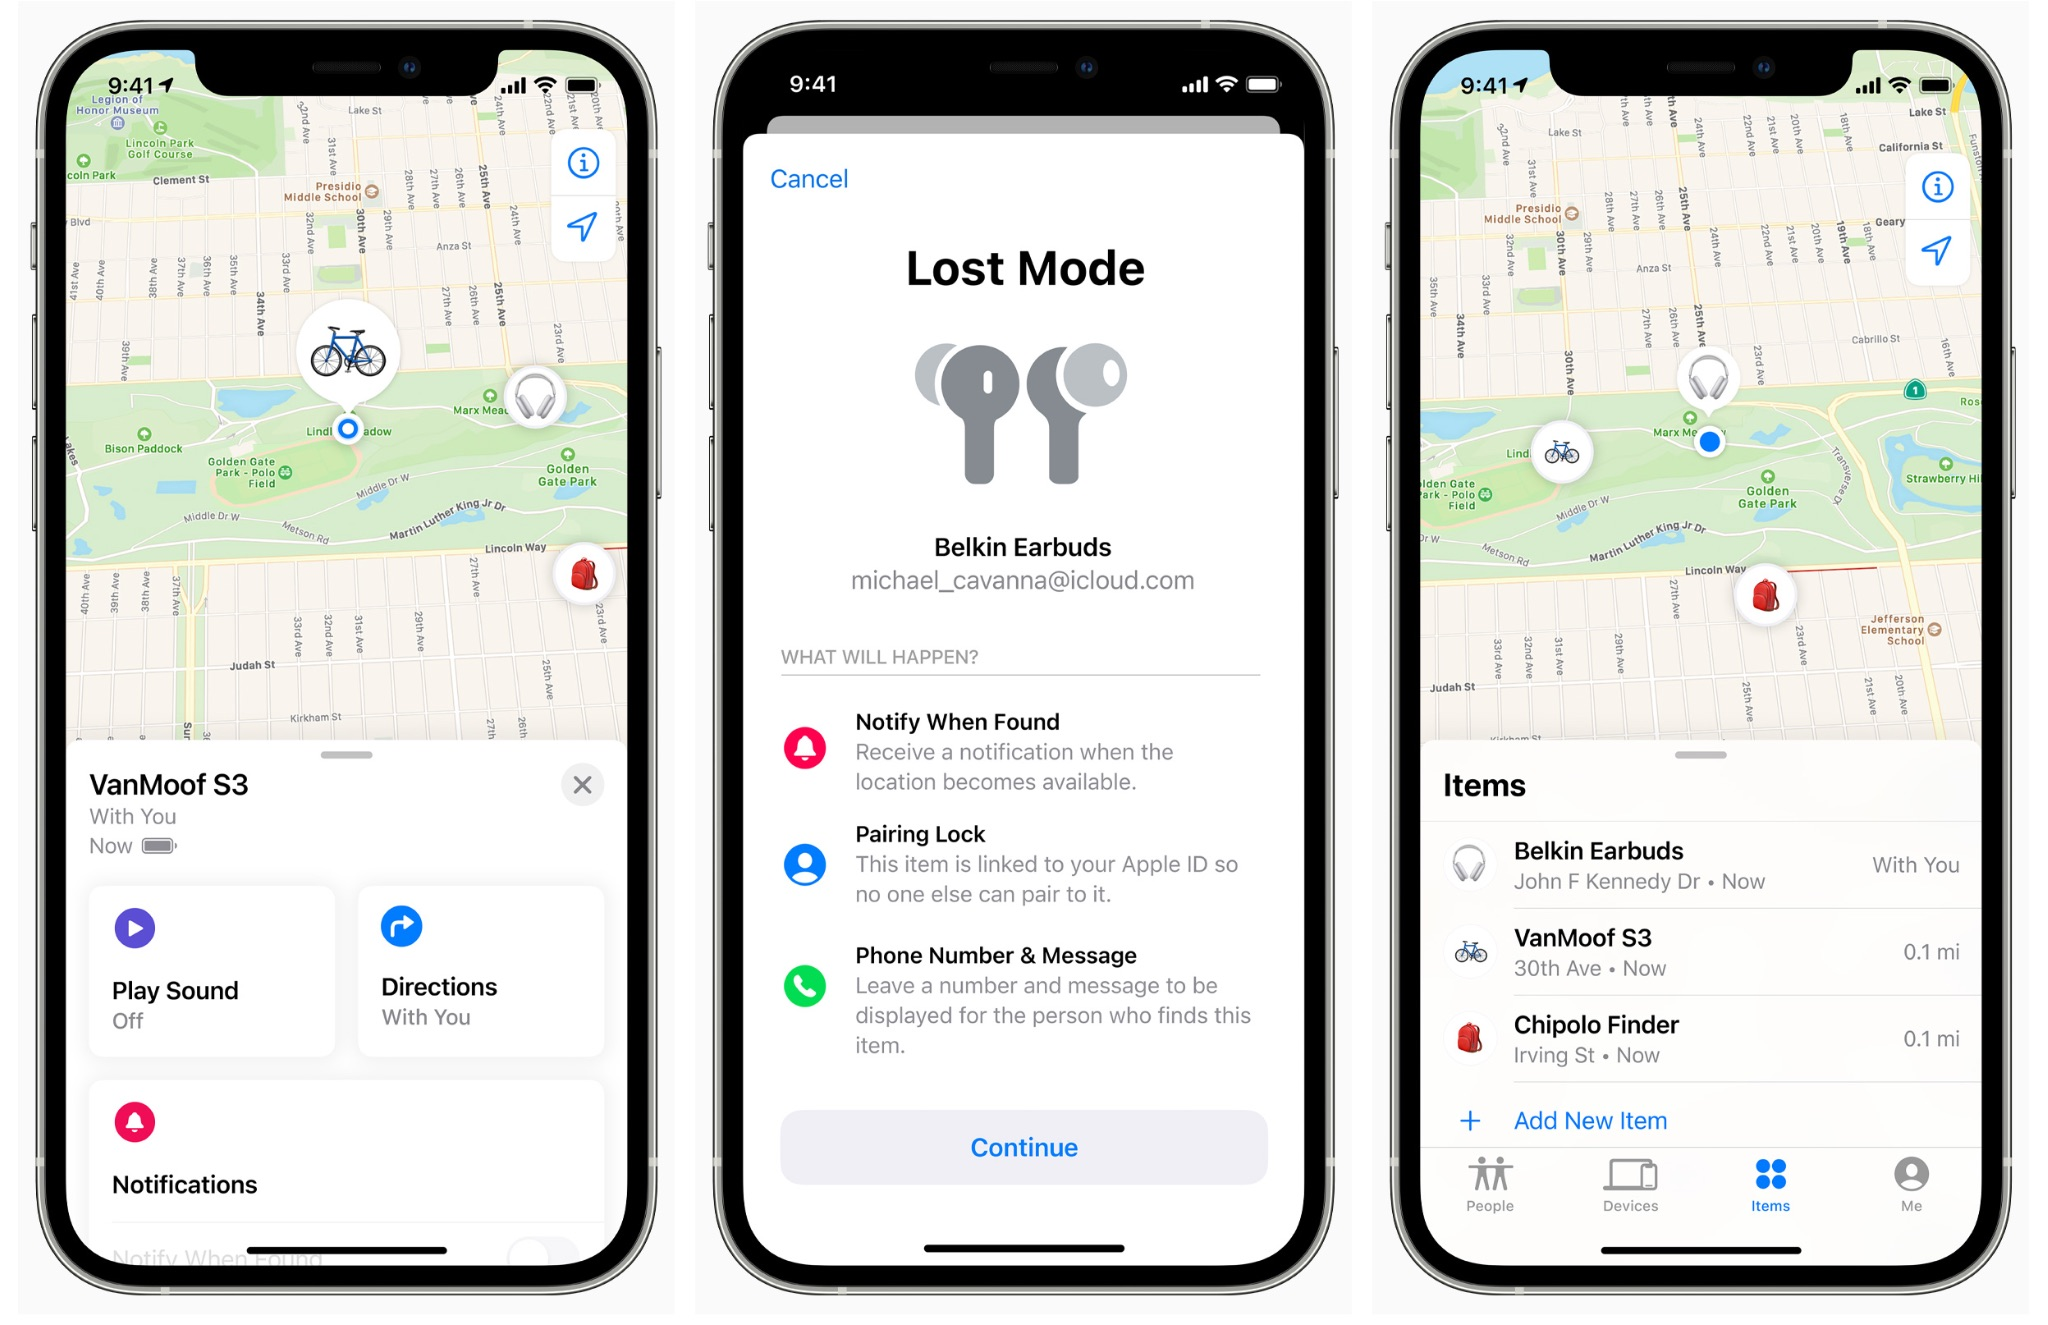
\includegraphics[width=.9\textwidth]{images/findmy.jpg}
	\caption{FindMy screenshots.}
	\label{findmy2}
\end{figure}

\subsection{Functioning}
%As for the functioning, we will use the content of \cite{Mayo_2021,Itani_2021,Clover_2022,OBoyle_2021} to describe the entire process. 
Now, we will descrive the entire functioning process; first of all we want to register our products within the application; in case of a non-accessory item, it will automatically be inserted in the \textit{Devices} section. In case of accessories, like AirTag, you need to manually add them using the \textit{Items} section.

Now you should be able to localize online devices from the map; in case of a close AirTag you can also use the \textit{Precision finding} to locate the object using U1 chip, as represented in Figure \ref{findmy1}. The technology fuses input from the iPhone's camera, ARKit, accelerometer and gyroscope in order to guide the user to their AirTag using a combination of sound, haptics, and visual feedback. 

\begin{figure}[t]
	\centering
	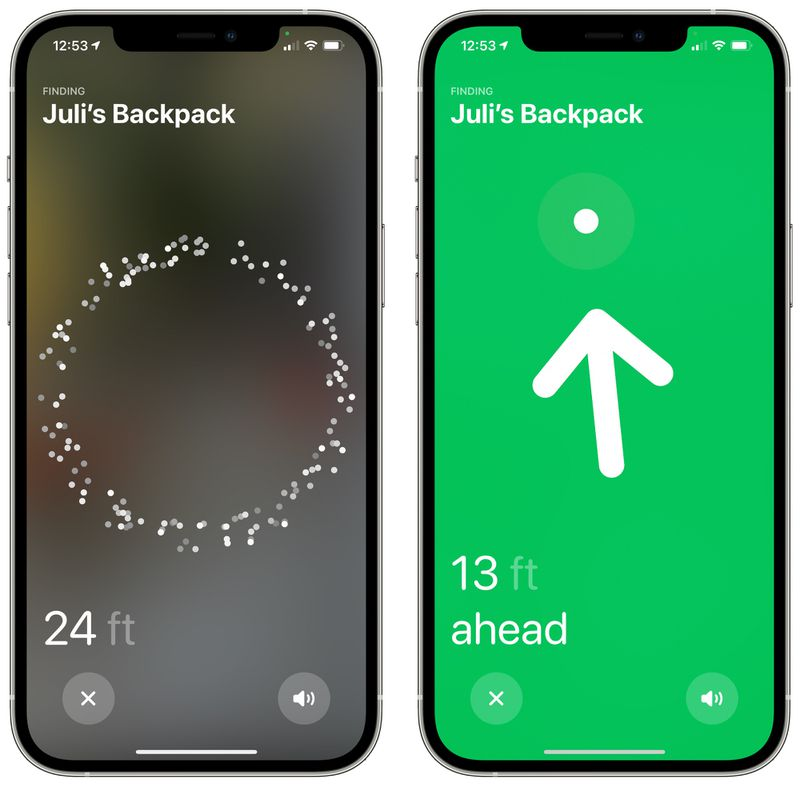
\includegraphics[width=.6\textwidth]{images/airtag-precision-finding-2.jpg}
	\caption{Precision Finding.}
	\label{findmy1}
\end{figure}

In case of a stolen device, you can always activate \textit{Lost Mode}; it will send you a notification as soon as the iphone is relevated, which means that if the phone will be connected to a network or via BLE to other Apple devices the owner will receive a message from FindMy containing the position of the device. Also, in this modality, all the registered cards in Apple Pay will be temporaneously disabled.

This technology seems already pretty useful, but if a device is powered off how can it be localized? With the introduction of iOS 15 and the U1 chips, Apple claimed that even a U1-based iPhone can be localized even when turned off if and only if the Bluetooth is turned on. From Apple: With iOS 15, your iPhone is still traceable through the Find My network even when the device is powered off. 
It seems that with iOS 15, the phone is not really fully powered off, it stays in a low-power state and acts like an AirTag, allowing any nearby iOS device to pick up the Bluetooth signal and send back its location.
This also means if the iPhone runs out of battery during the day, the owner still has a chance of finding its location for several more hours. In fact, Apple says the location tracking will even keep working whilst the phone is reset to factory settings with Activation Lock enabled. What about other devices, like Macbooks? Since Apple has not commented on the matter, the author conducted some tests and discovered that even machines with high specifications lack the U1 chip and are therefore not localizable when turned off. 

As already written, AirTags can be tracked through the \textit{Items} tab and have all of the tracking features available to Apple devices like iPhones and iPads. There's a Lost Mode, and AirTags can also take advantage of the Find My network that allows them to be tracked by billions of iPhones, iPads, and Macs when they're out of range of the owner devices. The only way to stop an AirTag from being fully detectable is to remove the CR2032 coin battery (or when it fully discharges).

\subsection{Security analysis}
In this section we will analyze the security measures implemented in FindMy to increase the safety of the architecture. Let us add some more details in the process of localizing an object.
\subsubsection{Preliminars definitions}
Let us first define a few terms in accordance with \cite{whocanfind}:
\begin{itemize}
  \item \textit{Owner Devices}: Owner devices share a common Apple ID and can use the Find My application on macOS, iOS and ipadOS to search for any devices of the same owner.
  \item \textit{Lost Devices}: Devices that determine to be in a lost state start sending out BLE advertisements with a public key to be discovered by finder devices. Apple devices are considered to be lost when they lose Internet connectivity. Third-party accessories \cite{gadget} are small battery-powered devices that can be attached to a personal item and are set up through an owner device. Accessories determine to be lost when they lose their BLE connection to the owner device.
  \item \textit{Finder Devices}: Finder devices form the core of the FindMy network. As of 2023, only iPhones and iPads with a GPS module are offering finder capabilities. Finder devices can discover lost devices and accessories by scanning for BLE advertisements. Upon receiving an advertisement, a finder creates an end-to-end encrypted location report that includes its current location and sends it to Apple’s servers. We will see what are the contents of the report.
  \item \textit{Apple’s Servers}: Apple’s servers store the location reports submitted by finder devices; only owner devices can fetch those reports and decrypt them locally.
\end{itemize}
\subsubsection{Workflow}
An online device can report its location to the user via iCloud. Find My works offline by sending out short range BLE signals from the missing device that can be detected by other Apple devices in use nearby. Those nearby devices then relay the detected location of the missing device to iCloud so users can locate it in the Find My app while protecting the privacy and security of all the users involved. An example of the previous workflow is represented in figure \ref{process}.

\begin{figure}[]
	\centering
	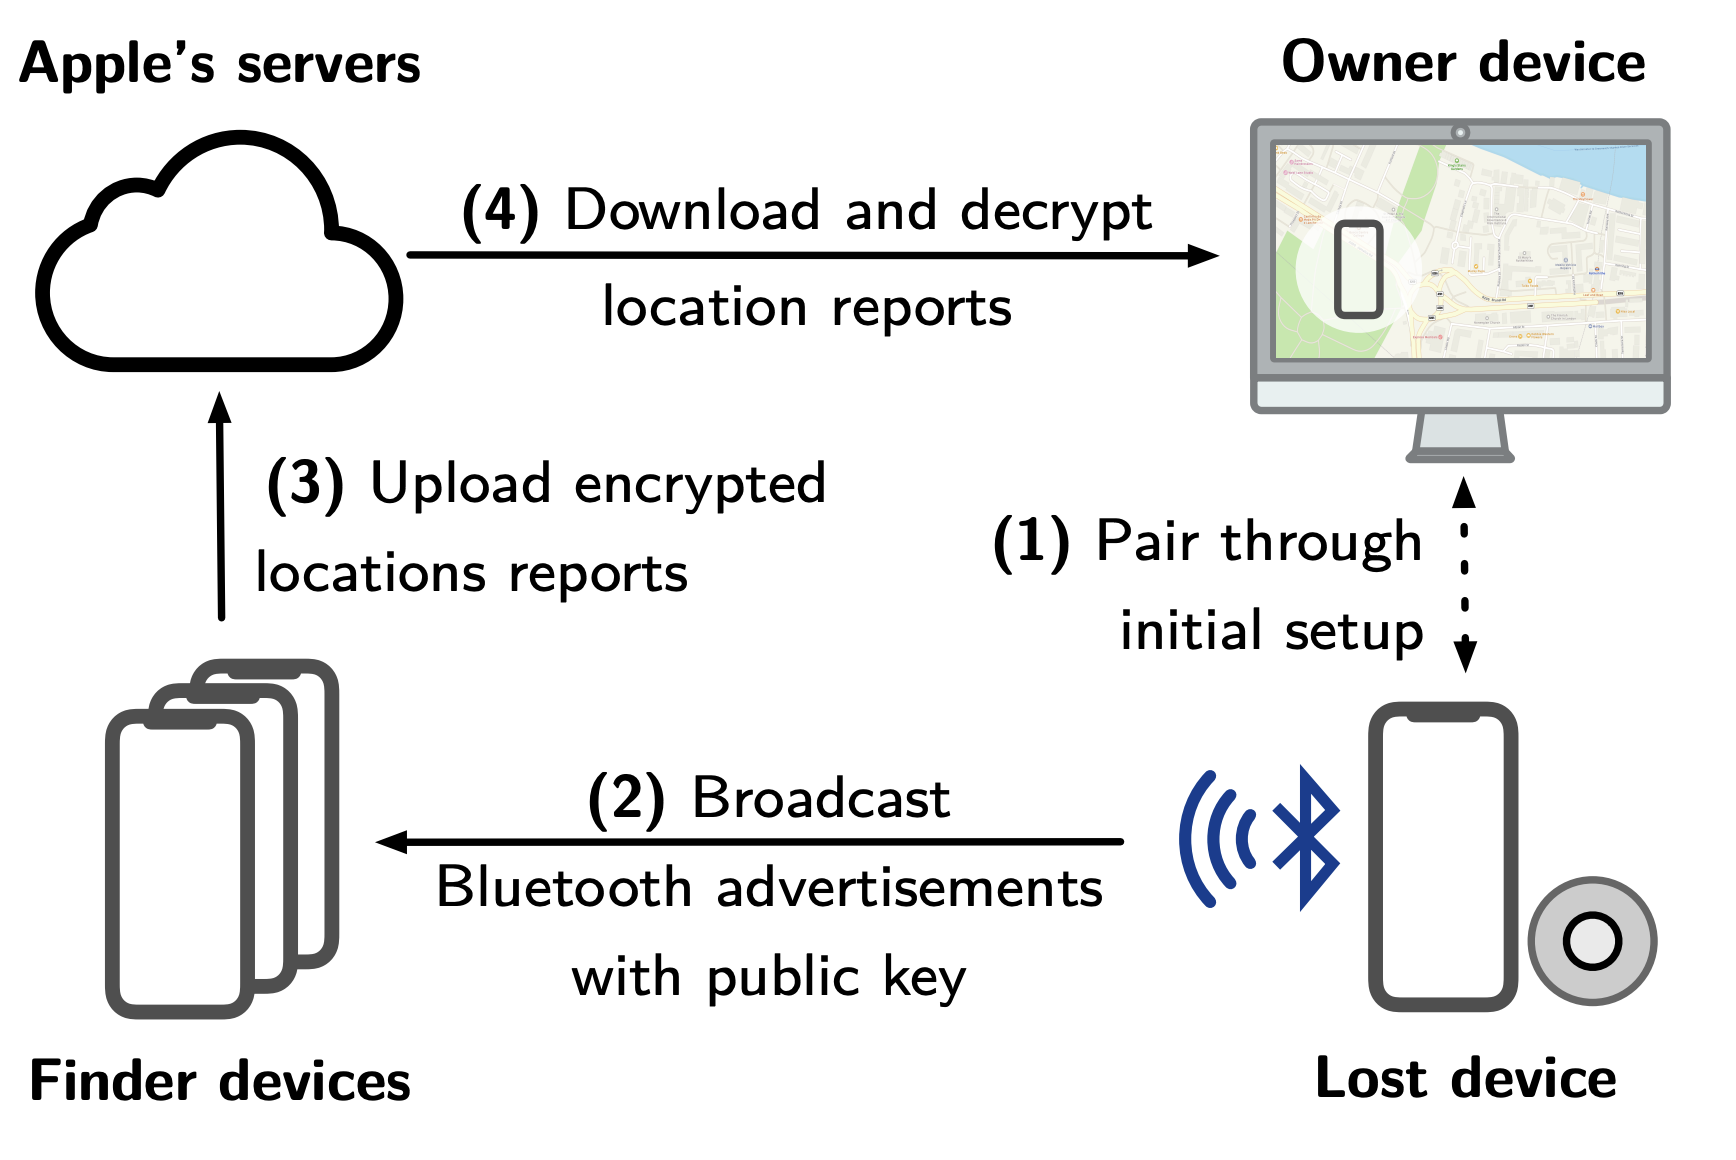
\includegraphics[width=.5\textwidth]{images/process.png}
	\caption{FindMy workflow (image from \cite{whocanfind}).}
	\label{process}
\end{figure}
All finder devices regularly scan for FindMy advertisements.
The finder creates and uploads an encrypted position report to Apple's servers whenever it receives a packet in the FindMy advertising format; finder devices are likely to use less energy and bandwidth because they gather reports over time and transfer them in batches on a regular basis. The evaluation done in \cite{whocanfind} discovered that the median time from generating to uploading a location report is 26 min and the delay can increase to several hours if the finder device is in a low power mode.

\subsubsection{Cryptography}
We will now delve more in the used Cryptography protocols. 
\paragraph{Advertisement keys}\label{keys}
FindMy utilises Elliptic Curves \cite{ec}; according to \cite{aps,whocanfind} the process to generate \textit{advertisement keys} is the following:
\begin{enumerate}
  \item Each owner device generates a private/public key pair
  $(d_0, p_0)$ on the NIST $P-224$ curve and a $32$-byte symmetric key $SK_0$ that together form the master beacon key. Those keys are never sent out via BLE and are used to derive the rolling advertisement keys included in the BLE advertisements. Note that device tracking is hard since rolling keys can be deterministically derived if and only if one knows the initial input keys $(d_0, p_0)$ and $SK0$.
  \item Advertisement keys $(d_i,p_i)$ are iteratively calculated as follows using the ANSI X.963 key derivation function $KDF$ \cite{ANSI} with $SHA-256$ \cite{sha} and a generator $G$ of the NIST P-224 curve:
  \begin{align}
    SK_i &= KDF(SK_{i-1},\ 'update',\ 32) \\
    (u_i, v_i) &= KDF(SK_i,\ 'diversify',\ 72) \\
    d_i &= (d_0 * u_i) + v_i \\
    p_i &= d_i * G
  \end{align}
  where Equation $(1)$ derives a new symmetric key from the last used symmetric key with 32 bytes length. Equation $(2)$ derives the so-called “anti-tracking” keys $u_i$ and $v_i$ from the new symmetric key with a length of $36$ bytes each. Finally, Eqs. $(3)$ and $(4)$ create the advertisement key pair via EC point multiplication using the anti-tracking keys and the master beacon key $d_0$.
\end{enumerate}

\paragraph{Key synchronization}
To download and decode location information, the advertisement keys must be accessed by all owner devices. In order to synchronize the master beacon keys, FindMy uses iCloud to encrypt a property list file in the Galois/Counter mode of the Advanced Encryption Standard (AES-GCM) \cite{gcm}. The file's decryption key is kept in the iCloud keychain underneath the label “Beacon Store”.

\paragraph{Encryption}
The BLE advertisements sent out by a lost device contain an EC public key $p_i$. A finder
device that receives such an advertisement determines its current location and encrypts the location with $p_i$. OF employs the Elliptic Curve Integrated Encryption
Scheme (ECIES), which performs an ephemeral Elliptic Curve Diffie-Hellmann (ECDH) key exchange to derive a shared secret used to encrypt the report. According to \cite{whocanfind}, the finder’s encryption algorithm works as follows:
\begin{enumerate}
  \item Generate a new ephemeral key $(d', p')$ on the NIST P-224 curve for a received FindMy lost advertisement.
  \item Perform ECDH using the ephemeral private key $d'$ and the advertised public key $p_i$ to generate a shared secret.
  \item Derive a symmetric key with ANSI X.963 $KDF$ on the shared secret with the advertised public key as entropy and SHA-256 as the hash function.
  \item Use the first 16 bytes as the encryption key $e'$.
  \item Use the last 16 bytes as an initialization vector $IV$.
  \item Encrypt the location report under $e'$ and the $IV$ with AES-GCM. 
\end{enumerate} 
The ephemeral public key $p'$ and the authentication tag of AES-GCM are part of the uploaded message. All location reports are identified by an $ID$ which is the SHA-256 hash of $p_i$, as we can see in figures \ref{comparison}.

\paragraph{Decryption}
An owner device that retrieves encrypted location reports follows the inverse of the encryption procedure:
\begin{enumerate}
  \item The owner device selects the proper advertisement keys $(d_i, p_i)$ based on the hashed $p_i$ of the location report.
  \item It performs the ECDH key exchange with the finder’s ephemeral public key $p'$ and the lost device’s private key $d_i$ to compute the symmetric key $e'$ and the $IV$.
  \item Now, the owner can use $e'$ and $IV$ to decrypt the location report.
\end{enumerate}

\begin{figure}
	\centering
	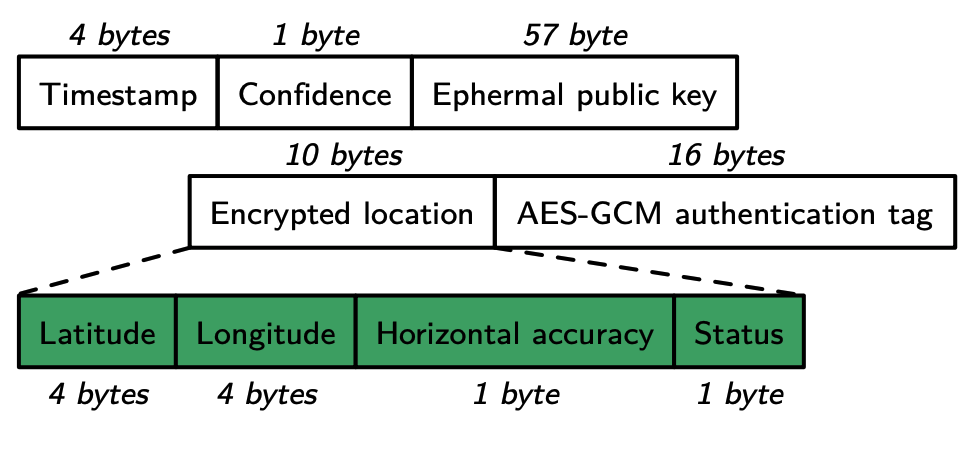
\includegraphics[width=0.5\textwidth]{images/packet.png}\hfill 
	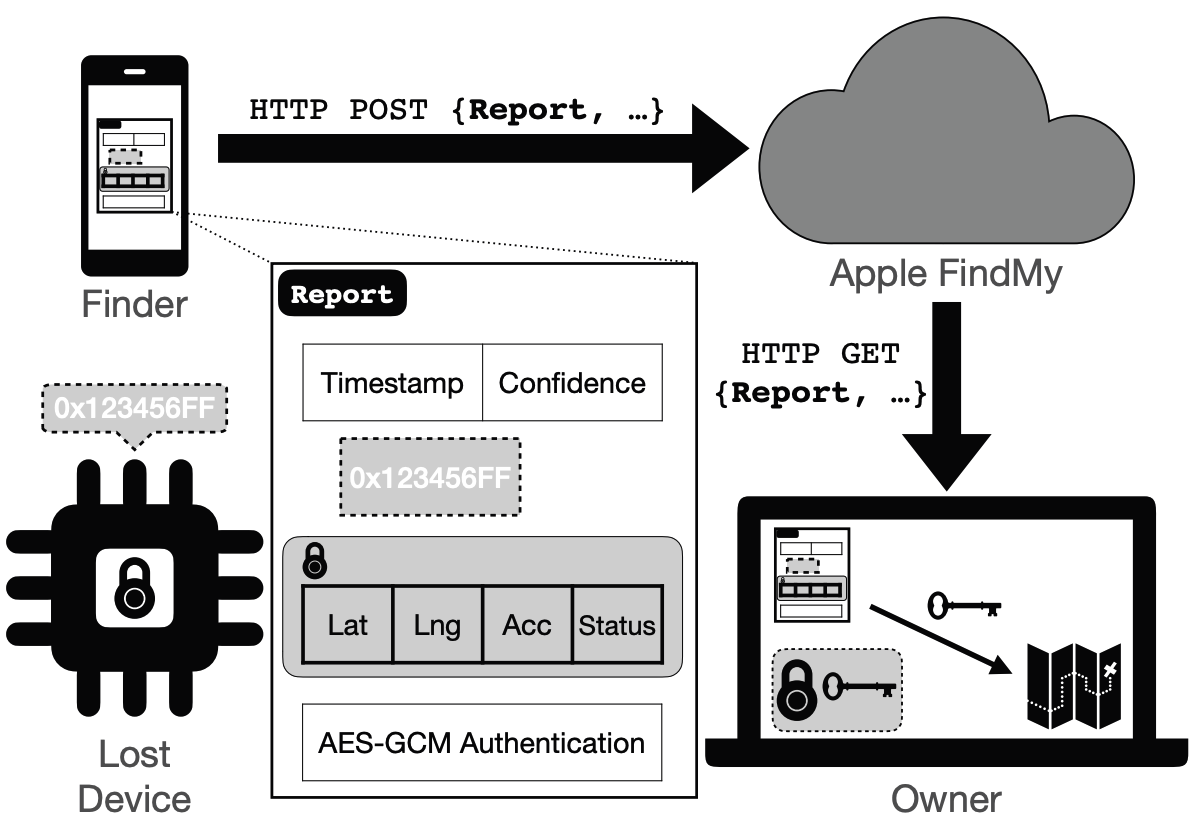
\includegraphics[width=0.5\textwidth]{images/findmysec.png}
	\caption{(a) Binary format of a location report \quad (b) Example of sent payload (images from \cite{whocanfind},\cite{airguard}).}
	\label{comparison}
\end{figure}


\section{AirTag}\label{sec:at}
An AirTag is a small tracking device developed and sold by Apple; it is intended to assist users in finding and monitoring objects that are easily misplaced or lost, such as wallets, bags, and keys.
\subsection{Overview}
 By connecting to compatible Apple devices (iPhones, iPads, and Macs) through Bluetooth, the AirTag enables users to locate the linked object and, subsequently, the AirTag itself using the Find My app. In order to help with lost item recovery, the gadget has capabilities including accurate location tracking, proximity notifications and a Lost Mode. Its design prioritizes privacy and security, safeguarding user data through the use of encryption and anonymization. Support for the AirTag was introduced in iOS 14.5 and Apple lists as compatible all the devices that support iOS 14 and iPadOS.
\subsection{Architecture}
First of all we will analyze the architecture of this product; informations have been reverse engineered by Adam Catley in \cite{reverse}. We will cover both the hardware and the software aspects of this kind of devices.
\subsubsection{Software analysis}
As for the software part, we can identify various states in which AirTag can be; we will now quickly present all of them.
\begin{itemize}
  \item \textit{Not registered}: When the AirTag is brand new, has been reset, or has been removed from the FindMy network. Waits to be connected to while advertising itself every 33ms.
  \item \textit{Initialisation}: The AirTag is being registered to an Apple ID and a public/private key pair is generated and shared between the AirTag and the connected iOS device.
  \item \textit{Connected}: The owner’s device is in range. No broadcasts occur.
  \item \textit{Disconnected}: The owner’s device is out of range. Broadcasts identity every 2000ms.
  \item \textit{Out of sync}: Happens when an AirTag reboots while separated from its owner’s device. Acts like Disconnected but absolute time is lost so events are relative to time since power-up. Identity resets to initial value.
  \item \textit{Lost}: Occurs 3 days after Disconnected or Out of sync begin. Moves to Waiting for motion every 6 hours.
  \item \textit{Waiting for motion}: Samples the accelerometer every 10 seconds until motion is detected.
  \item \textit{Sound alert}: A command to play a noise is received from either a connected device or by detecting motion. Lasts a maximum of 20 seconds.
  \item \textit{Precision finding}: Triggered by the owner’s device while in Connected. Is overridden by Sound alert.
\end{itemize}
As we will see in section \ref{hw}, the AirTag uses a NFC antenna to allow anyone who finds an AirTag to potentially identify the owner, even if they have an Android device. The tag can only be read when the AirTag is powered by a battery and it contains a URL to uniquely identify the AirTag, depending on its current state. There are some parameters that are attached to the URL, used to identify the device; we will briefly present them. Keep in mind that all of the following parameters are fixed for a single unit, even after power cycles, long runtime, resets and modes.
\begin{itemize}
  \item \textit{pid}: Product ID for AirTag.
  \item \textit{b}: Something related to the battery.
  \item \textit{pt}: UWB Precision Tracking version.
  \item \textit{fv}: Firmware version.
  \item \textit{dg}: Something related to diagnostic.
  \item \textit{z}: Unknown.
  \item \textit{bt}: Bluetooth address; will be present only when Unregistered.
  \item \textit{st}: Serial number of the tag (the one printed on the device under the battery); will be present only when Unregistered.
  \item \textit{bp}: Bluetooth protocol version; will be present only when Unregistered.
\end{itemize}
In the \textbf{Unregistered} state, the stored URL has the following format:
\url{https://found.apple.com/airtag?pid=5500&b=00&pt=004c&fv=00100e10&dg=00&z=00&bt=A0B1C2D3E4F5&sr=ABCDEF123456&bp=0015}

Once the device is \textbf{registered}, the parameters \textit{bt, sr, bp} will be removed and replaced with a single anonymous identifier \textit{pi}, which is the only parameter that changes at least every 15 minutes when the Bluetooth address and/or the advertising data changes. It is likely the current P-224 public key $p_i$ presented in \ref{keys} or the SHA-224 of it. 


The device operates on a schedule designed to optimize its functionality:
at 4:00 am every day, it updates its BLE address and public key, ensuring secure communication channels.
Advertisement data is refreshed every 15 minutes, guaranteeing that nearby devices receive the most current information.
Should it become separated from its owner's device for three days, the device enters a lost mode, activating specific features to aid in recovery efforts.
While in this lost mode and detecting movement, the device emits a noise every 6 hours to alert nearby individuals.
To conserve energy while remaining responsive, the accelerometer is sampled every 10 seconds when waiting for movement.
Upon detecting motion, the accelerometer sampling frequency increases to every 0.5 seconds for 20 seconds, providing detailed tracking data.
When away from its owner's device, the device transmits BLE advertisement signals every 2 seconds, enhancing its detectability.
Finally, in close proximity to its owner's device, the device establishes a BLE connection interval of 1 second, ensuring efficient communication and responsiveness.
\subsubsection{Hardware analysis}\label{hw}
As for the hardware part, an important aspect comes to the light: all of the used components, apart from Apple's U1 UWB chip, are off the shelf, as we can see in Figure \ref{img:pcb}.
Each AirTag has three antennas: one for BLE that works at 2.4 GHz, one for NFC at 13.56 MHz and finally the UWB one at 6.5-8 GHz.
The outer plastic shell, which serves as a diaphragm, is adhered to the voice coil. When the coil is energized, the fixed magnet causes it to move back and forth, creating sound and serving as the speaker.
Whether the voice coil is connected or not, the AirTag functions in the same way.
If motion is detected, the speaker will loudly beep for up to 20 seconds after being apart from its owner's device for three days. After that, it will be silent for the following six hours before watching for movement once more.
\begin{figure}[ht]
	\centering
	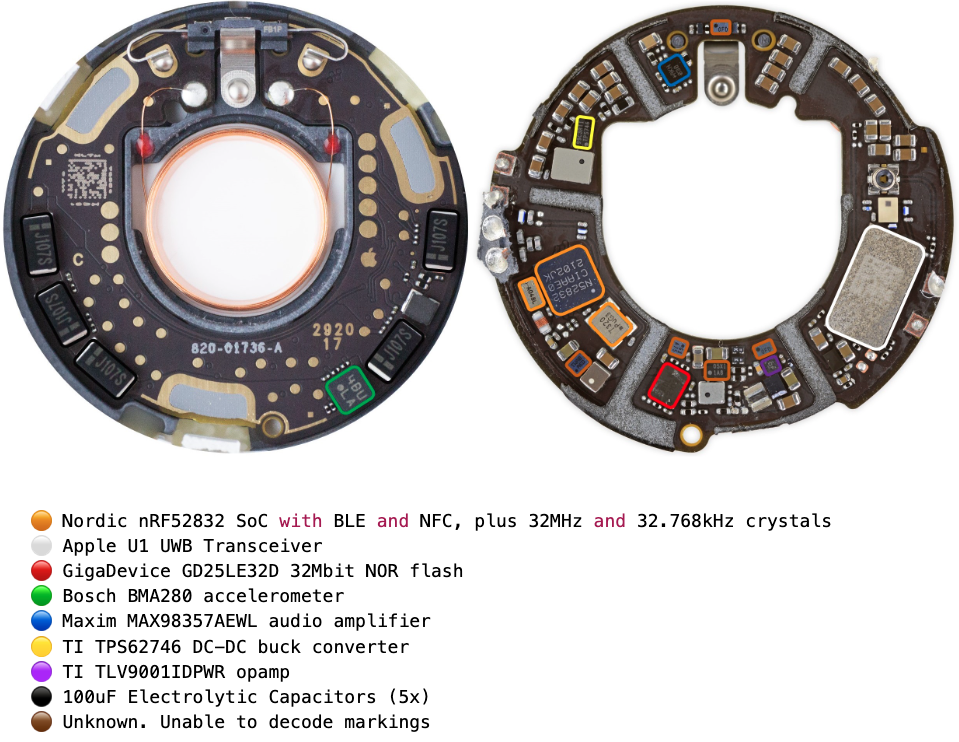
\includegraphics[width=\textwidth]{images/pcb.png}
	\caption{PCB overview (image from \cite{reverse}). }
	\label{img:pcb}
\end{figure}

\subsection{Security Analysis}\label{sec}
Security-wise, there is a lack of basic security controls in this kind of devices; in fact, none of the data in the AirTag is protected from tampering or disclosure.
\subsubsection{Vulnerabilities}
\paragraph{Side-channel attacks}
The Nordic nRF52832 has the function Access Port Protection\cite{nordicsemi} that is used to disable access to the Debug Port through SWD and prevent reading out the internal memory; however, according to \cite{side}, this mechanism is vulnerable to side channel attacks and can be bypassed through voltage glitching. Consequentially, it is possible to extract Bluetooth pairing keys to connect to the owner’s phone or run (on the AirTag) a custom firmware since Apple does not check the signature of it (the firmware).

\paragraph{Insecure Storage}The GD25LE32D 32Mbit NOR flash is not encrypted, as we can see in \cite{tweet}; also the nRF52832 does not have any secure storage functionality. In this case we don't know if this is a real vulnerability since we do not know whether the FindMy private key-pair is stored inside the AirTag.

\paragraph{Replay attacks}The only way to identify an AirTag is to use its public key, which is transmitted via BLE advertising packets; this identification does not require authentication. These IDs can be recorded and replayed by any nearby BLE device to mimic the appearance of the real AirTag. Let's see an example: an attacker steals a personal item containing an AirTag and subsequently record the current public identity before removing the battery. At this point, the identity can be relayed to any BLE device in a decoy location to give the owner a false search area to recover their property.
\subsubsection{Anti-stalking measurements}
An important aspect that has emerged with the AirTags is the stalking problem. Stalking using AirTags refers to the potential misuse of Apple's AirTag tracking devices to monitor and track individuals without their consent; these small devices are designed to help users locate misplaced items. However, due to their small size and long battery life, AirTags could potentially be used for nefarious purposes, such as stalking. An individual could secretly place an AirTag on someone's belongings and then use the Find My app to monitor their movements in real-time. Since AirTags are designed to be difficult to detect, the victim may not realize they are being tracked for an extended period.

Apple has implemented measures to prevent the misuse of AirTags, including alerts and notifications for when an unknown AirTag is detected near a user's device, as well as features like Precision Finding, which can help users locate unwanted AirTags. The first line of defense in the event that someone plants an AirTag on a victim belongings might be an alert to his iPhone indicating the presence of a foreign AirTag. Apple built the iPhone-AirTag connection to do this in two ways: either when you get to the place that your iPhone's machine learning intelligence has detected as home (or when you manually record it as home) or after the AirTag has stuck with you for a certain "continuous" period of time that Apple deems sufficient to be considered abnormal. This seems perfect, however if the victim has a non Apple device, such as an Android Phone this could be a problem. To prevent this problem, Google and Apple collaborated to develop Unknow Tracker Alerts, which is a feature that was announced during the Google I/O 2023 opening presentation.

Additionally, AirTags are designed to emit sound if they have been separated from their owner for an extended period, potentially alerting the victim to the presence of the tracking device. More precisely, three days following separation is when sound alerts begin; even in that case, they only occur once motion is identified and only for a maximum of 20 seconds. After that, the AirTag remains silent for a maximum of 20 seconds every six hours while it waits for movements. The problem with this is that three days can be enough to study the victim's routine and after that period, it is likely to make noise for a maximum of 40 seconds a day during a normal commuting schedule. Movement is likely to coincide with a noisy environment while travelling or muffled by objects touching the white casing, meaning that the victim won't realize it. According to \cite{server}, the frequency and duration of sounds can be adjusted from Apple server side, meaning that Apple can increase both of them to avoid situations in which the victim is unable to ear the sounds.

However, despite these safeguards, the potential for AirTags to be used for stalking remains a concern; in fact, a problem is that the voice coil can be disconnected without disassembly. This means that the AirTag will function as normal without emitting sounds, thus an attacker can easily modify an AirTag and be unknowingly placed in someone’s possessions to track a target’s location without them being audibly notified of its presence.
\subsection{Useful applications}
Some useful applications can be the following:
\begin{itemize}
  \item Travel: AirTags can be beneficial for travelers. They can attach AirTags to their luggage, making it easier to identify and track their bags during travel. 
  \item Pet Tracking: While not explicitly designed for pets, some users have found AirTags useful for tracking their pets; by attaching an AirTag to a pet's collar owners can monitor their pet's location and quickly locate them if they wander off.
  \item Child Safety: Similarly to pets, AirTags can offer an additional layer of security for keeping track of children in crowded or unfamiliar places; by attaching an AirTag to a child's backpack or clothing, parents can monitor their child's whereabouts and receive alerts if they stray too far.
  \item Vehicle Tracking: AirTags can also be used to track vehicles, such as bicycles, motorcycles or cars in the same way as the two above.
  \item People with Dementia Tracking: People with Alzheimer's or another form of dementia can lose their ability to recognize familiar places, so it's not uncommon for them to wander off and get lost and confused; in this case we can use AirTags to be sure about where they are.
\end{itemize}

\subsection{Mods}
After some Internet researchs, the author discovered that the AirTag has been modified in certain ways. For instance, in \cite{telecomando} A. Catley has attached the AirTag to a remote controller and is powering the AirTag components using the host's battery. This could be very useful in situations in which the remote controller gets lost in the house; thanks to Precision Finding, the owner can find it easily. Figure \ref{img:controller} shows the final result.
Now, imagination knows no bounds, and there are always innovative ways to utilize AirTags.
\begin{figure}[]
	\centering
	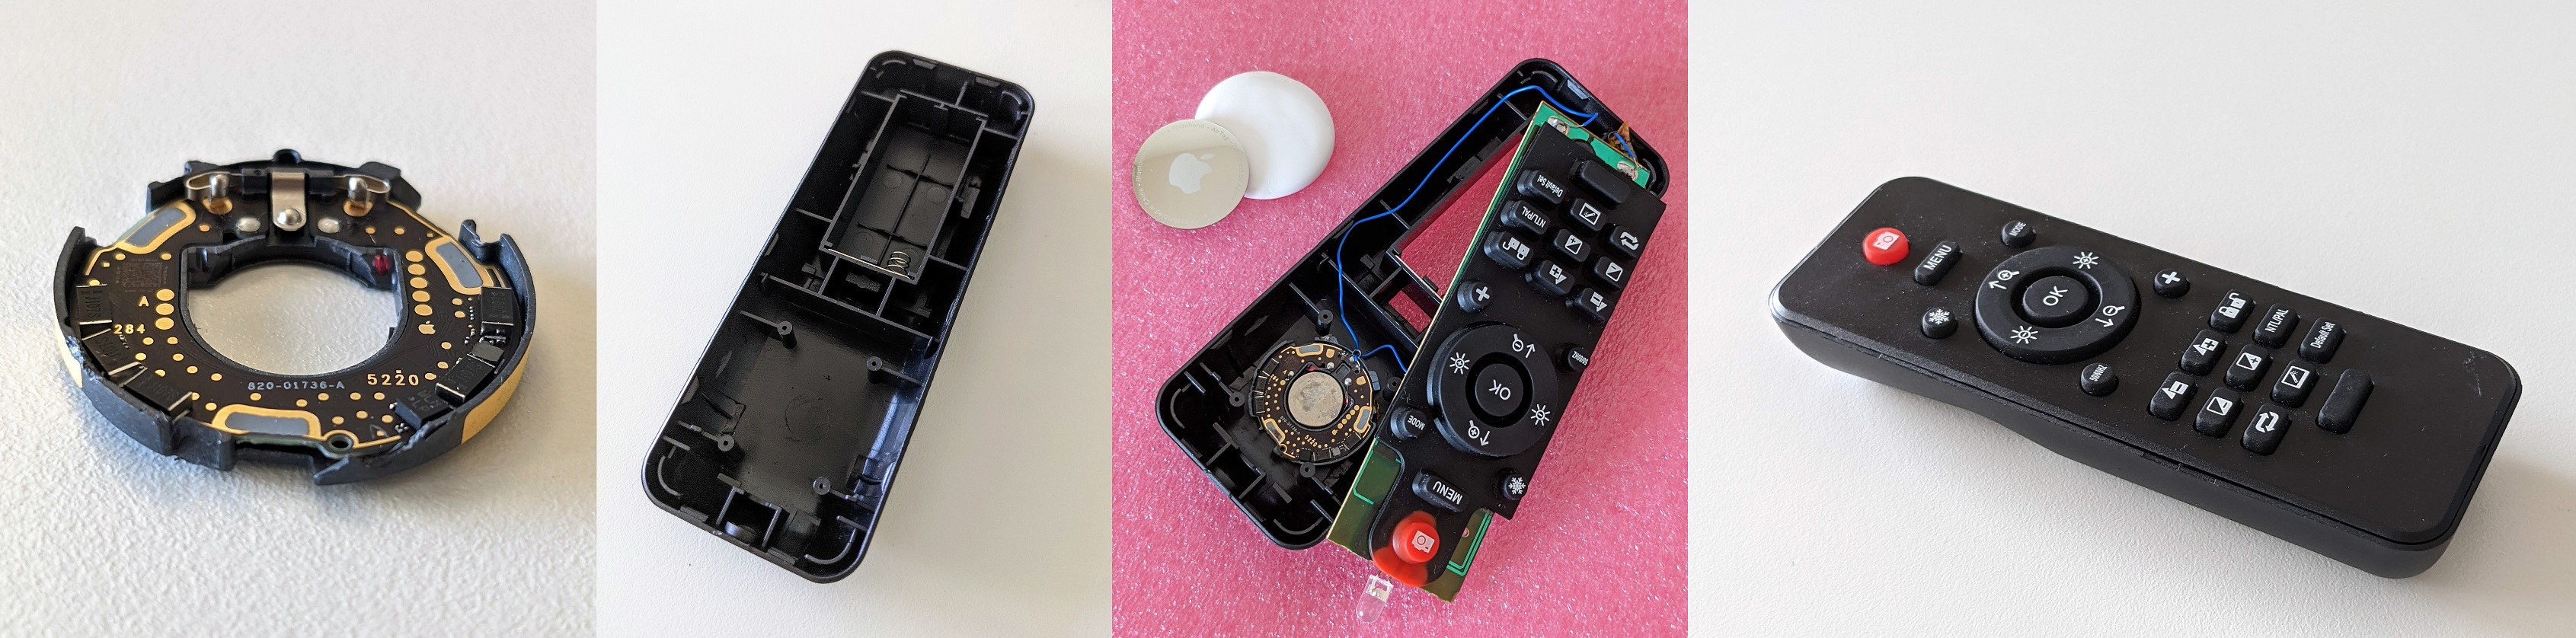
\includegraphics[width=\textwidth]{images/remote.jpg}
	\caption{AirTag inside a remote control (images from \cite{reverse}).}
	\label{img:controller}
\end{figure}

\section{Conclusion}
In conclusion, the paper provided a comprehensive exploration of various technological aspects. Section \ref{sec:intro} offered a broad overview of the themes to be addressed, setting the stage for deeper investigation. Section \ref{sec:uwb} delved into UWB technology, offering not only a general introduction but also a detailed analysis of its security implications, particularly in the context of Apple's implementation.

Progressing to Section \ref{sec:find}, the focus shifted to the FindMy network. Here, the discussion began with an overview, followed by a practical example to illustrate its operation. Subsequently, an examination of FindMy's security measures was conducted, shedding light on the intricacies of its encryption protocols.

Section \ref{sec:at} centered on AirTag, starting with an overview before analyzing its architectural components, encompassing both software and hardware aspects. This was followed by an in-depth security analysis, uncovering vulnerabilities inherent in these devices that could potentially be exploited by malicious entities. Despite their cost-effectiveness and utility, it was evident that improvements in security measures, such as the introduction of authentication protocols during key exchange, were necessary to fortify their defenses against replay attacks, as discussed in \ref{sec}.
Lastly, the paper briefly report practical applications of these technologies, including an example where modifications were applied to adapt them to alternative contexts. 

\printbibliography
\nocite{*}

\end{document}